\begin{figure}
    \begin{subfigure}{0.3\textwidth}
        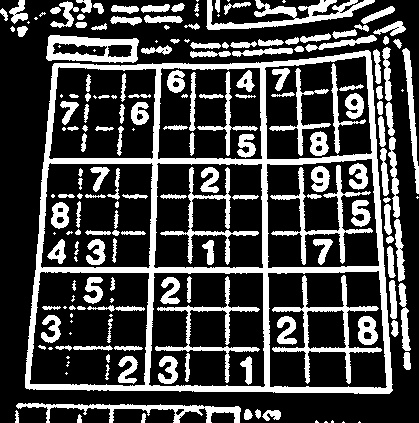
\includegraphics[width=\linewidth] {../../test/threshold/1.jpg}
        \caption{Input image}\label{fig:sht_example:a}
    \end{subfigure}\hfill
    \begin{subfigure}{0.3\textwidth}
        \centering
        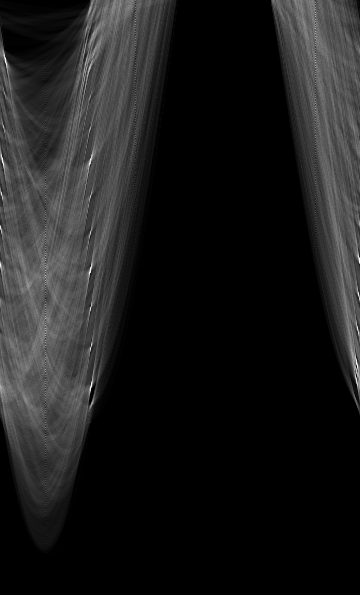
\includegraphics[height=\linewidth] {../../packages/js-benchmarks/img/seq.png}
        \caption{Accumulator}\label{fig:sht_example:b}
    \end{subfigure}\hfill
    \begin{subfigure}{0.3\textwidth}
        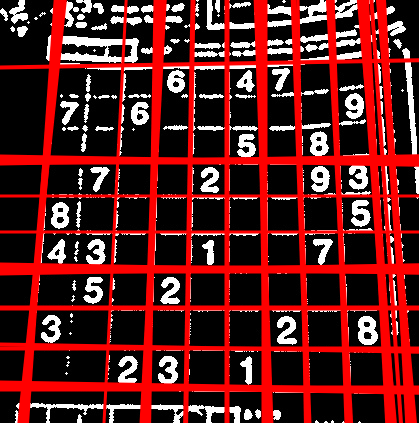
\includegraphics[width=\linewidth] {img/sht_result.png}
        \caption{Detected lines}\label{fig:sht_example:c}
    \end{subfigure}
    \caption{Input image (419x421), accumulator and visualized result of sequential SHT algorithm in \textit{non-LUT} variant ($S_\theta = 1, S_\rho=1$).}\label{fig:sht_example}
\end{figure}
